%%%%%%%%%%%%%%%%%%%%%%%%%%%%%%%%%%%%%%%%%
% Short Sectioned Assignment LaTeX Template Version 1.0 (5/5/12)
% This template has been downloaded from: http://www.LaTeXTemplates.com
% Original author:  Frits Wenneker (http://www.howtotex.com)
% License: CC BY-NC-SA 3.0 (http://creativecommons.org/licenses/by-nc-sa/3.0/)
%%%%%%%%%%%%%%%%%%%%%%%%%%%%%%%%%%%%%%%%%

% \documentclass[paper=a4, fontsize=11pt]{scrartcl} % A4 paper and 11pt font size
\documentclass[11pt, a4paper]{book}
\usepackage[T1]{fontenc} % Use 8-bit encoding that has 256 glyphs
\usepackage[utf8]{inputenc}
\usepackage{fourier} % Use the Adobe Utopia font for the document - comment this line to return to the LaTeX default
\usepackage{listings} % para insertar código con formato similar al editor
\usepackage[spanish, es-tabla]{babel} % Selecciona el español para palabras introducidas automáticamente, p.ej. "septiembre" en la fecha y especifica que se use la palabra Tabla en vez de Cuadro
\usepackage{url} % ,href} %para incluir URLs e hipervínculos dentro del texto (aunque hay que instalar href)
\usepackage{graphics,graphicx, float} %para incluir imágenes y colocarlas
\usepackage[gen]{eurosym} %para incluir el símbolo del euro
\usepackage{cite} %para incluir citas del archivo <nombre>.bib
\usepackage{enumerate}
\usepackage{hyperref}
\usepackage{graphicx}
\usepackage{tabularx}
\usepackage{booktabs}

\usepackage[table,xcdraw]{xcolor}
\hypersetup{
	colorlinks=true,	% false: boxed links; true: colored links
	linkcolor=black,	% color of internal links
	urlcolor=cyan		% color of external links
}
\renewcommand{\familydefault}{\sfdefault}
\usepackage{fancyhdr} % Custom headers and footers
\pagestyle{fancyplain} % Makes all pages in the document conform to the custom headers and footers
\fancyhead[L]{} % Empty left header
\fancyhead[C]{} % Empty center header
\fancyhead[R]{Gestión de ofertas publicadas en canales de Discord y Telegram} % My name
\fancyfoot[L]{} % Empty left footer
\fancyfoot[C]{} % Empty center footer
\fancyfoot[R]{\thepage} % Page numbering for right footer
%\renewcommand{\headrulewidth}{0pt} % Remove header underlines
\renewcommand{\footrulewidth}{0pt} % Remove footer underlines
\setlength{\headheight}{13.6pt} % Customize the height of the header

\usepackage{titlesec, blindtext, color}
\definecolor{gray75}{gray}{0.75}
\newcommand{\hsp}{\hspace{20pt}}
\titleformat{\chapter}[hang]{\Huge\bfseries}{\thechapter\hsp\textcolor{gray75}{|}\hsp}{0pt}{\Huge\bfseries}
\setcounter{secnumdepth}{4}
\usepackage[Lenny]{fncychap}


\begin{document}

	% Plantilla portada UGR
	\begin{titlepage}
\newlength{\centeroffset}
\setlength{\centeroffset}{-0.5\oddsidemargin}
\addtolength{\centeroffset}{0.5\evensidemargin}
\thispagestyle{empty}

\noindent\hspace*{\centeroffset}\begin{minipage}{\textwidth}

\centering

\includegraphics[width=0.9\textwidth]{logos/logo_ugr.jpg}\\[1.4cm]

\textsc{ \Large TRABAJO FIN DE GRADO\\[0.2cm]}
\textsc{ GRADO EN INGENIERÍA INFORMÁTICA}\\[1cm]

{\Huge\bfseries Título \\}
\noindent\rule[-1ex]{\textwidth}{3pt}\\[3.5ex]
{\large\bfseries Subtítulo }
\end{minipage}

\vspace{2.5cm}
\noindent\hspace*{\centeroffset}
\begin{minipage}{\textwidth}
\centering

\textbf{Autor}\\ {Jerónimo Chaves Caballero}\\[2.5ex]
\textbf{Director}\\ {Juan Julián Merelo Guervós}\\[2cm]

\includegraphics[width=0.3\textwidth]{logos/etsiit_logo.png}\\[0.1cm]
\textsc{Escuela Técnica Superior de Ingenierías Informática y de Telecomunicación}\\
\textsc{---}\\
Granada, Junio de 2023
\end{minipage}
\end{titlepage}


	% Plantilla prefacio UGR
	\thispagestyle{empty}

\begin{center}
{\large\bfseries Título \\ Subtítulo }\\	%FIXME: Cambiar Título / Subtítulo cuando lo tengamos
\end{center}
\begin{center}
Jerónimo Chaves Caballero\\
\end{center}

%\vspace{0.7cm}

\vspace{0.5cm}
\noindent\textbf{Palabras clave}: \textit{software libre}
\vspace{0.7cm}

\noindent\textbf{Resumen}
	

\cleardoublepage

\begin{center}
	{\large\bfseries Same, but in English}\\	%FIXME: Cambiar contenido por el Título / Subtítulo en inglés
\end{center}
\begin{center}
	Jerónimo Chaves Caballero\\
\end{center}
\vspace{0.5cm}
\noindent\textbf{Keywords}: \textit{open source}, \textit{floss}
\vspace{0.7cm}

\noindent\textbf{Abstract}


\cleardoublepage

\thispagestyle{empty}

\noindent\rule[-1ex]{\textwidth}{2pt}[4.5ex]

D. \textbf{Juan Julián Merelo Guervós}, Profesor del  departamento de Ingeniería de Computadores, Automática y Robótica.

\vspace{0.5cm}

\textbf{Informo:}

\vspace{0.5cm}

Que el presente trabajo, titulado \textit{\textbf{Chief}},	%FIXME: Cambiar 'Chief' por el título definitivo del trabajo
ha sido realizado bajo mi supervisión por \textbf{Jerónimo Chaves Caballero}, y autorizo la defensa de dicho trabajo ante el tribunal
que corresponda.

\vspace{0.5cm}

Y para que conste, expiden y firman el presente informe en Granada a Junio de 2023.

\vspace{1cm}

\textbf{El/la director(a)/es: }

\vspace{5cm}

\noindent \textbf{(Juan Julián Merelo Guervós)}

\chapter*{Agradecimientos}






	% Índice de contenidos
	\newpage
	\tableofcontents

	% Índice de imágenes y tablas
	\newpage
	\listoffigures

	% Si hay suficientes se incluirá dicho índice
	\listoftables 
	\newpage

	% Introducción 
	\chapter{Introducción}

Este proyecto es software libre, y está liberado con la licencia GPL 3\cite{gplv3}.

La intención de este proyecto es solucionar el siguiente problema:

\textbf{Resumir las ofertas de un canal de Telegram o Discord en los precios actuales y el mínimo alcanzado para un videojuego.}

En nuestro caso, estamos basándonos sobre todo en uno de los canales más utilizados para este tipo de problema: el canal Ofertas Juegos en Telegram.

Teniendo esto en cuenta, debemos de encontrar una solución adecuada para esto que sea rápida de desarrollar, pero fácilmente escalable en
caso de que queramos partir de esta base para crear algo más grande.


	% Estado del arte
	\chapter{Estado del arte}

Como se ha mencionado anteriormente, hay bastantes maneras de buscar ofertas de 
videojuegos, ya sea por portales web como \url{chollometro.com}, o por canales de 
comunicación, teniendo como ejemplo específico a \url{ofertasjuegos.es} en lo que 
respecta a canales de Telegram.

Es cierto que podemos buscar ofertas en ambos métodos (sobre todo en el ejemplo 
puesto para portales web dedicados a ello), pero aun así no podemos saber cuándo 
hay una oferta de algo que nos interesa al momento si no estamos revisando todo el 
rato el portal web, o puede que se pierda en todos los mensajes que se envían en el 
canal de Telegram.

Es por esto que este proyecto pretende coleccionar las ofertas desde un mismo sitio 
para que sea fácil explorar por ellas, buscando específicamente lo que nos interesa 
y sin la necesidad de pasar por todas esas ofertas que son irrelevantes para 
nosotros.

Esto ayuda a que el usuario pueda centrarse solamente en un único sitio y no tener 
la necesidad de estar entrando en varios portales web o canales de Telegram para 
encontrar ofertas.

Para el desarrollo del proyecto, necesitamos obtener la información de los 
distintos sitios de ofertas. En este caso, vamos a centrarnos primero en obtener 
los datos desde Telegram, que cuenta con una API para poder obtener los mensajes de 
un canal o chat, además de su uso extendido para los famosos bots de la aplicación.

Por tanto, es fácil encontrar librerías que permiten utilizar la API de Telegram de  
una manera más sencilla. Dentro de la propia documentación de Telegram 
podemos encontrar una lista curada 
\footnote{Bot API Library Examples \url{https://core.telegram.org/bots/samples}} de 
los que tienen más librerías.

Teniendo esto en cuenta, vamos a categorizar los lenguajes para elegir la mejor 
opción para el proyecto.

Las categorías serían:

\begin{itemize}
    \item \textbf{Facilidad de aprendizaje/entendimiento}: Queremos un lenguaje que 
    si no lo conocemos, podamos adaptarnos rápidamente a él.
    \item \textbf{Comunidad}: Si contamos no solamente que el lenguaje sea de
    rápida adaptación, sino que además tenga una comunidad extensa, nos será más 
    fácil resolver nuestras dudas.
    \item \textbf{Eficiencia del lenguaje}: Además de los puntos anteriores, es 
    importante elegir un lenguaje que sea eficiente en cuanto a recursos, ya que 
    podemos encontrarnos con que consuma demasiada memoria o haga que nuestra 
    factura sea un poco más alta de lo que esperábamos. Esto ya se ha explorado y 
    se puede encontrar una lista curada \cite{eficiencia} de los lenguajes.
\end{itemize}

Teniendo en cuenta estas categorías y la lista que nos proporcionan en la 
documentación de Telegram, hemos decidido utilizar Go como lenguaje de programación 
para nuestro proyecto.
	
	\chapter{Planificación}

La planificación de un proyecto llega a ser una de las partes más cruciales del 
desarrollo de este y de su éxito. Es el proceso mediante el cual se definen los 
objetivos, se establecen las tareas y se asignan los recursos necesarios para 
llevar a cabo la creación de un software de manera eficiente y efectiva.

En este capítulo vamos a exponer las distintas metodologías que 
vamos a utilizar tanto para las tareas como para el desarrollo además de dónde se 
puede encontrar el repositorio y las herramientas utilizadas para seguir las 
metodologías.

\section{Metodologías utilizadas}

Decidiendo las distintas metodologías que queremos seguir durante el proyecto, se 
han seleccionado tres metodologías que se llegan a usar en el desarrollo ágil: 
\textbf{Kanban}, \textbf{Desarrollo Dirigido por Pruebas} e \textbf{Integración 
Continua}.

Primero, \textbf{Kanban} \cite{kanban} es una metodología de desarrollo ágil que se 
emplea para visualizar y gestionar el flujo de trabajo de un proyecto, basándose en 
tres tableros: tareas pendientes, en progreso y completadas. Las distintas tareas 
se representan en tarjetas, que vamos moviendo de un tablero a otro según el estado 
de estas.

Nosotros hemos añadido un cuarto tablero, donde pondremos que tareas están 
bloqueadas por otra tarea o proceso. Así, vemos de un vistazo que debemos de 
priorizar para que el proyecto avance (figura \ref{fig:tabla-kanban}).

\begin{figure}[h]
    \centering
    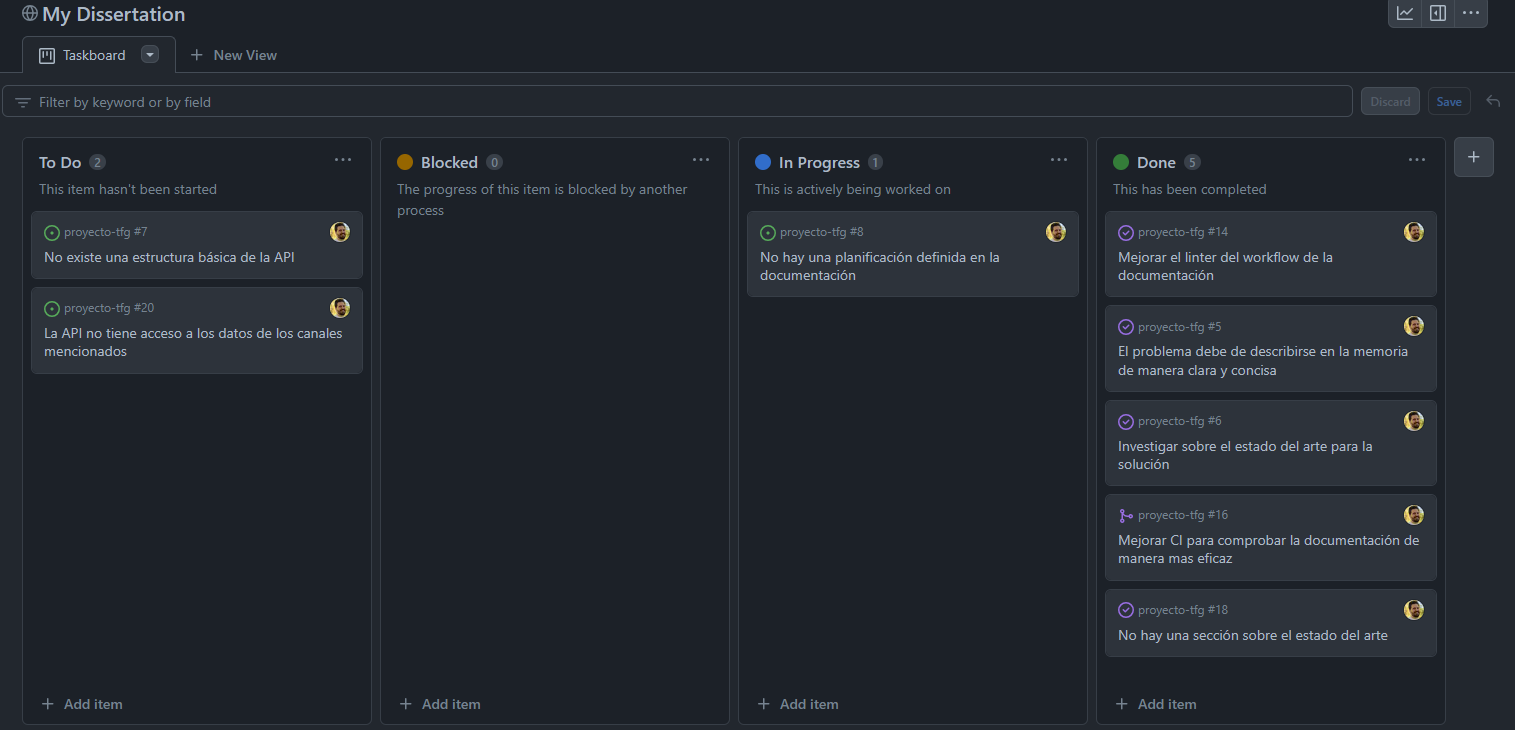
\includegraphics[scale=0.3]{figuras/github-projects-proyecto-tfg.png}
    \caption{Tablas Kanban dentro de GitHub Projects.}
    \label{fig:tabla-kanban}
\end{figure}

El \textbf{Desarrollo Dirigido por Pruebas} (\textbf{TDD}, en inglés \textbf{Test 
Driven Development}) \cite{tdd} es una práctica de desarrollo de software que se 
basa en crear primero las pruebas antes de implementar el código de la 
funcionalidad. Con esto, podemos conseguir tener el código más limpio y que se 
compruebe de manera fácil que el código funciona como indican los requisitos.

Por último, la \textbf{integración continua} (\textbf{CI}, en inglés 
\textbf{Continuous Integration}) \cite{ci} es una metodología de desarrollo de 
software que consiste en integrar los nuevos cambios en el código verificando 
previamente que estos cambios no rompen el código existente. Para llegar a esto, se 
aplicará lo siguiente:

\begin{enumerate}
    \item \textbf{Automatización de pruebas}: Las pruebas (que hemos mencionado 
    anteriormente) serán automatizadas en el flujo de trabajo.
    \item \textbf{Compilación automatizada}: Se compilará el código con los cambios 
    realizados para revisar que no hay problemas durante la compilación.
    \item \textbf{Despliegue automatizado}: Se desplegará el código en un entorno 
    para su acceso en el momento en el que lleguemos al producto mínimo viable.
\end{enumerate}

\section{Usuarios}

Para el desarrollo de este proyecto, se han definido los siguientes tipos de 
usuarios:

\begin{itemize}
    \item \textbf{Tribunal de evaluación}: Este trabajo de fin de grado será 
    evaluado por un grupo de profesores de la universidad y, por tanto, se debe de 
    asociar una memoria que contenga la explicación del proyecto.
    \item \textbf{Estudiante}: Cuenta con un presupuesto limitado. Puede preferir 
    comprar un mayor número de videojuegos con ese presupuesto o bien, comprar por 
    el que más interesado está a un precio menor de su precio de venta al público 
    (PVP) para ahorrar dinero.
    \item \textbf{Coleccionista}: El presupuesto es más elevado que el anterior 
    caso que hemos descrito. Le interesa más la disponibilidad de los videojuegos, 
    aunque también aprecia poder llevárselo por un precio menor.
\end{itemize}

\section{Historias de usuario}

Habiendo identificado los distintos usuarios que hemos encontrado, podemos 
desarrollar las historias de usuario relacionadas o casos de uso que se pueden 
desarrollar para este proyecto. Para ello, hemos definido las siguientes historias:

\subsection{[HU00] Generar una buena estructura en la memoria}

Como tribunal de TFG, necesito entender todos los términos que figuran en el TFG, 
entender claramente cuál es la aportación del estudiante, y los retos que ha 
superado. Y quiero verlo por escrito en un informe que esté correctamente escrito, 
tenga el formato correcto, y exprese claramente el trabajo realizado.

\textbf{Condiciones de satisfacción}:

\begin{itemize}
    \item La memoria debe de estar fácilmente accesible.
    \item La memoria debe de contener un estudio acerca del estado del arte.
    \item La memoria debe de contener información acerca de la metodología que se 
    esté utilizando.
    \item La memoria debe de contener la definición de los objetivos e historias de 
    usuario del proyecto.
    \item La memoria debe de estar correctamente escrita.
\end{itemize}

\subsection{[HU01] Buscar videojuegos por nombre}

Como estudiante/coleccionista, quiero poder buscar un videojuego por su nombre para 
obtener las distintas tiendas que lo venden y su precio, además de su enlace de 
compra para cada una.

Como tribunal de TFG, quiero conocer el desarrollo de la solución necesario para 
poder obtener la información de un videojuego por su nombre, para así poder 
evaluar al estudiante.

\textbf{Condiciones de satisfacción}:

\begin{itemize}
    \item La solución debe de poder buscar un videojuego por su nombre.
    \item La solución debe de poder obtener las distintas tiendas que venden el 
    videojuego.
    \item La solución debe de poder obtener el precio de cada tienda.
    \item La solución debe de poder obtener el enlace de compra del videojuego para 
    cada tienda.
    \item El desarrollo de la solución debe de estar correctamente explicado, tanto 
    la parte de desarrollo con código como las necesidades para implementarlo.
\end{itemize}

\section{Seguimiento del desarrollo}

Para el seguimiento del desarrollo del proyecto, hemos decidido usar Git como 
sistema de control de versiones y la plataforma GitHub para alojar el repositorio 
remoto del proyecto.

Lo bueno de GitHub es que, además, nos ofrece más herramientas para seguir las 
distintas metodologías que hemos mencionado anteriormente:

\begin{itemize}
    \item \textbf{GitHub Issues}: Con Issues podemos añadir nuestras tareas para el 
    proyecto para poder saber que hace falta llevar a cabo.
    \item \textbf{GitHub Milestones}: Con Milestones podemos agrupar las tareas que 
    hemos ido creando poco a poco y priorizar lo que se debe de hacer antes. 
    Además, con esto hemos podido adecuar un Producto Mínimo Viable (MVP en inglés) 
    con la Milestone 1. Si se quiere ver los distintos Milestones, se puede 
    mediante el siguiente enlace: 
    \url{https://github.com/jero-dev/proyecto-tfg/milestones}
    \item \textbf{GitHub Projects}: Con Projects podemos generar un tablero para 
    seguir la metodología Kanban y comprobar el estado de las tareas o issues que 
    están representadas por las tarjetas (figura \ref{fig:tabla-kanban}). El 
    proyecto se puede encontrar en el siguiente enlace: 
    \url{https://github.com/users/jero-dev/projects/1}
    \item \textbf{GitHub Actions}: Gracias a esta herramienta podemos automatizar 
    tanto la compilación como la ejecución de pruebas cada vez que se añadan 
    cambios. Por tanto, gracias a esto, podemos seguir la metodología de 
    integración continua durante el desarrollo.
\end{itemize}


	% Análisis del problema
	% 1. Análisis de requisitos
	% 2. Análisis de las soluciones
	% 3. Solución propuesta
	% 4. Análisis de seguridad
	\chapter{Análisis del problema}
 
Habiendo descrito ya el problema, vamos a analizarlo. Para ello, seguiremos el 
diseño dirigido por dominios (en inglés, Domain Driven Design o DDD) \cite{ddd} 
para identificar de manera correcta el dominio del problema y poder así 
concentrarnos totalmente en él.

\begin{itemize}
    \item \textbf{Dominio del problema:} Tenemos como dominio del problema la 
    gestión de ofertas y promociones de productos (aunque nos centremos en 
    videojuegos). Los conceptos (entidades) que hemos identificado son:
    \begin{itemize}
        \item \textbf{Producto:} Bien o servicio que se ofrece en el mercado.
        \item \textbf{Precio:} Cantidad de dinero que se asigna a un producto.
        \item \textbf{Oferta:} Reducción del precio de un producto por tiempo 
        limitado.
        \item \textbf{Tienda:} Establecimiento donde se venden productos.
    \end{itemize}
    Habiendo comentado acerca de usuarios, los ejemplos de usuario que vamos a 
    seguir para el desarrollo del proyecto son:
    \begin{itemize}
        \item \textbf{Estudiante:} Usuario que no tiene un gran presupuesto para 
        comprar los productos que quiere y desea estar informado de las ofertas que 
        le permitan adquirirlos.
        \item \textbf{Fanático o coleccionista:} Usuario que tiene bastante 
        presupuesto en comparación al usuario anterior, pero que prefiere obtener 
        el mayor número de productos posibles por el mismo precio.
    \end{itemize}
    \item \textbf{Agregados:} Estos son conjuntos de entidades y/o valores que se 
    tratan como una sola unidad. En este caso, podemos tener el agregado de 'oferta 
    de producto', que se compondría de las entidades 'producto', 'oferta' y 'tienda'.
    \item \textbf{Contexto delimitado:} Para centrarnos en el problema, tenemos que 
    delimitar el contexto del mismo. Aquí tenemos claro que el contexto es la 
    gestión de ofertas.
    \item \textbf{Servicios de dominio:} Los servicios de dominio encapsulan la 
    lógica de negocio que no pertenece a ninguna entidad o valor. Aquí podemos sacar 
    tres claros servicios de dominio: 'obtención de información', 'gestión de 
    productos' y 'gestión de ofertas'.
    \item \textbf{Eventos de dominio:} Estos son sucesos significativos que ocurren 
    dentro del dominio. Aquí primordialmente tendríamos dos eventos: el de 'oferta 
    disponible' y el de 'oferta expirada'.
\end{itemize}


	% Desarrollo bajo sprints: 
	% 	1. Permitir registros y login de usuarios
	% 	2. Desarrollo del sistema de incidencias
	% 	3. Desarrollo del sistema de denuncias administrativas y accidentes
	% 	4. Desarrollo del sistema de croquis
	%   5. Instalación de la aplicación de manera automática
	\chapter{Implementación}

La implementación del software se ha dividido en hitos. Estos, han sido definidos en GitHub
y cada uno de ellos contiene un grupo de \textit{issues} que se corresponden con las distintas
mejoras que se han ido incorporando al software a lo largo de su desarrollo.


	% Presupuesto

	% Conclusiones
	%\chapter{Conclusiones y trabajos futuros}



	% Trabajos futuros


	
	\newpage
	\bibliography{bibliografia}
	\bibliographystyle{plain}
	
\end{document}

